\documentclass[a4paper,11pt]{article}

%%%%%%%%%%%%%%%%%%%%%%%%%%%%%%%%%
%            ATENÇÃO            %
% NÃO ALTERE AS LINHAS A SEGUIR %
%%%%%%%%%%%%%%%%%%%%%%%%%%%%%%%%%

\usepackage[brazil]{babel}
\usepackage{float,graphicx,graphics,amssymb,amsfonts,newlfont,indentfirst}
\usepackage[centertags]{amsmath}
\usepackage{fancyhdr}
\usepackage{ragged2e}
\usepackage{geometry}
\geometry{top=0cm,bottom=2cm,left=3cm,right=2cm}
\usepackage[normalem]{ulem}
\pagestyle{fancy}
\usepackage{url}
\usepackage{color}
\usepackage[font+=small,leftmargin=4cm,rightmargin=0cm,indentfirst=false]{quoting}
%\fancyfoot{} %retira número das páginas do rodapé
\renewcommand{\rmdefault}{ptm}
\renewcommand{\sfdefault}{ptm}
\renewcommand{\ttdefault}{ptm}

\lhead{ERMAC, Volta Redonda -- RJ, 2023}

\fancypagestyle{capa}{%
	\fancyhead{}%
	\rhead{\textit{Trabalho apresentado no ERMAC, Volta Redonda -- RJ, 2023.}%
	\vspace*{11pt}}%
}

\usepackage{mathptmx} % Fonte Times em fórmulas

\headheight 10mm
\oddsidemargin 2.0mm
\evensidemargin 2.0mm
\topmargin -10mm
\textheight 240mm
\textwidth 160mm
\headsep 5mm
\parindent 1mm


%%%%%%%%%%%%%%%%%%%%%%%%%%%%%
% MODIFIQUE DAQUI EM DIANTE %
%%%%%%%%%%%%%%%%%%%%%%%%%%%%%

% pacotes adicionais
%\usepackage{algorithm}
\usepackage[pdftex]{hyperref} %permite resaltar texto
\hypersetup{colorlinks,citecolor=black,filecolor=black,linkcolor=black,urlcolor=black} %setup de hyperref
\bibliographystyle{unsrt}
\bibliographystyle{abntex2-alf}

\begin{document}

\centering{{\Large{\bf Herramienta para la simulacion del crecimiento de tumores en diversas regiones del cuerpo humano en 3 dimensiones.}}

\begin{flushright}{\it
\vspace*{5mm}
Carlos Carret Miranda\\
Universidad de la Habana\\
carlos.carret@estudiantes.matcom.uh.cu

\vspace*{5mm}
\underline{ Reinaldo Rodríguez Ramos}\\
Departamento de Matem\'aticas, Facultad de Matem\'aticas y Computaci\'on, Universidad de La Habana, Cuba y PPG-MCCT, Universidade Federal Fluminense, Volta Redonda, Rio de Janeiro, Brazil.\\
reinaldo@matcom.uh.cu y reinaldorr@id.uff.br

\vspace*{5mm}
Panters Rodríguez Bermúdez\\
Departamento de Ciências Exatas, Universidade Federal Fluminense, Volta Redonda, Rio de Janeiro, Brazil\\
pantersrb@id.uff.br

% se necessário, adicione mais autores como nos blocos acima
}\end{flushright}


\setcounter{equation}{0} % NÃO modifique esta linha


\thispagestyle{capa}
\justifying{
{\noindent \bf Resumo: }{\small{%
	%RESUMO
	El cancer es una enfermedad que se caracteriza por el crecimiento descontrolado de células anormales en el cuerpo, es una enfermedad compleja y multifacética que ha desafiado a los investigadores y médicos durante décadas. La capacidad de visualizar y entender el crecimiento de los tumores puede proporcionar una valiosa comprensión de cómo se desarrolla y se propaga el cáncer, lo que puede llevar a mejoras significativas en el diagnóstico, tratamiento y prevención del cáncer. La herramienta de simulación tridimensional del crecimiento de tumores que estamos desarrollando es un paso importante en este sentido. Permite la visualización detallada del crecimiento de los tumores en diferentes partes del cuerpo humano, lo que puede proporcionar una valiosa comprensión de cómo se desarrolla y se propaga el cáncer. Además, la capacidad de esta herramienta para simular el crecimiento de tumores en diferentes partes del cuerpo significa que puede ser utilizada para estudiar una amplia gama de tipos de cáncer. Esta herramienta utiliza un autómata celular y una red de mundo pequeño para crear las conexiones entre las células, permitiendo una representación más precisa de la estructura de los organos y los tumores. Además, permite cargar configuraciones y parámetros desde archivos externos, lo que aporta una gran flexibilidad a la herramienta y permite adaptar la simulación a las necesidades específicas de cada caso. Para la renderización en 3D, se utiliza la técnica de Marching Cubes, que permite una representación tridimensional detallada y precisa de los tumores. 
}}

\vskip 0.2cm  % NÃO modifique esta linha


{\small{ %PALAVRAS-CHAVE
\noindent{\bf{Palavras-chave:}} Automata Celular, Marching Cubes, 3D, cancer, tumor
}}
}

%%%%%%%%%%%%%%%%%%%%%%%%%%%%%
%%%%%%%%%%%%%%%%%%%%%%%%%%%%%

\section*{Introdução}

El desafío de representar matemática, física y computacionalmente fenómenos biológicos requiere de una sinergia interdisciplinaria de expertos en dichos campos. Esta colaboración interdisciplinaria enriquece el método experimental que se usa tradicionalmente en las ciencias biológicas con la implementación de modelos matemáticos, que sirven como una herramienta para formular y comprobar hipótesis, orientando investigaciones experimentales y afinando el modelo a través de los resultados obtenidos.~\cite{2}

El cáncer es una enfermedad que afecta a una gran cantidad de seres vivos y se caracteriza por la presencia de un grupo de células anormales que crecen sin control, ignorando las normas de la división celular. Afecta de forma especial al ser humano donde su aparición y desarrollo constituye un peligro para la vida. La malignidad del cáncer es variable y depende de la velocidad de crecimiento de las células cancerígenas, la capacidad de estas últimas de propagarse a otros tejidos y la posibilidad de reaparecer una vez que son removidas quirúrgicamente.
El propósito de este tipo de investigación es alcanzar un entendimiento más profundo de los procesos biológicos a través de un ciclo iterativo de teoría y experimentación. Además, los modelos matemáticos pueden ser empleados para asistir en la concepción y diseño de estrategias terapéuticas, proporcionando una visión más precisa y personalizada del tratamiento de cada paciente.

En el caso de este proyecto, se emplea un autómatas celular y una red de mundo pequeño para modelar las interacciones entre las células, lo que proporciona una representación más precisa del crecimiento tumoral. Los parámetros y configuraciones pueden ser cargados desde archivos externos, ofreciendo una gran flexibilidad en la adaptación de la simulación a las necesidades específicas de cada caso.

La técnica de Marching Cubes se utiliza para la renderización en 3D, proporcionando una visualización detallada y precisa de los tumores. Esta visualización puede proporcionar una comprensión valiosa de cómo se desarrolla y se propaga el cáncer, lo que puede ser esencial para el desarrollo de terapias y tratamientos efectivos. La visualización resultante puede proporcionar una comprensión valiosa de cómo se desarrolla y se propaga el cáncer. Al visualizar el crecimiento del tumor en tres dimensiones, los médicos y científicos pueden obtener una mejor comprensión de la evolución del tumor y cómo puede afectar a los tejidos circundantes. Esta información puede ser esencial para el desarrollo de terapias y tratamientos efectivos para el cáncer


\section*{Submissão}

\textbf{Automata Celular}

En esta secci\'on se concibe el modelo de aut\'omatas celulares que se presenta en este trabajo. Se comienza definiendo formalmente un aut\'omata celular~\cite{5}.

Un aut\'omata celular es una tupla $(\mathcal{L}; \mathcal{N}; \mathcal{E}; \mathcal{R})$ que se compone de los siguientes elementos representativos:
\begin{itemize}
\item [$\mathcal{L}$:] Es un conjunto potencialmente infinito de c\'elulas.
\item [$\mathcal{N}$:] $\mathcal{L} \times \mathcal{L} \rightarrow \lbrace 0,1 \rbrace$ es una funci\'on de vecindad, que puede ser vista como una relaci\'on, usualmente reflexiva y sim\'etrica, entre las c\'elulas. Esta funci\'on muestra qu\'e pares de c\'elulas son vecinas, o sea, la geometr\'ia de la organizaci\'on celular.
\item [$\mathcal{E}$:] Es un conjunto de estados. A cada c\'elula del conjunto $\mathcal{L}$ se le asigna un estado asociado en cada instante de tiempo.
\item [$\mathcal{R}$:] $\mathcal{E}^{|\mathcal{N}(v)|} \rightarrow \mathcal{E}$ es una funci\'on de transici\'on definida localmente. Esta funci\'on es el n\'ucleo de la din\'amica de un aut\'omata celular, y com\'unmente se expresa mediante reglas que definen el estado de la c\'elula en el siguiente instante de tiempo a partir del estado de las c\'elulas vecinas. El conjunto que contiene el estado de las c\'elulas vecinas se obtiene mediante la funci\'on $\mathcal{N}(v)$, que se define en~\ref{1}.
\end{itemize}

Los conjuntos $A^n(G)$ y $A^d(G)$ agrupan las aristas del grafo que corresponden a conexiones inmediatas y distantes, respectivamente. Estos conjuntos cumplen con las siguientes propiedades:
\begin{subequations}
\begin{equation}
A^n(G) \cup A^d(G) = A(G),
\end{equation}
\begin{equation}
A^n(G) \cap A^d(G) = \emptyset.
\end{equation}
\end{subequations}
Estas propiedades indican que los subconjuntos de aristas $A^n(G)$ y $A^d(G)$ constituyen una partición del conjunto de aristas $A(G)$

En base a los conjuntos de vértices $V(G)$ y de aristas $A(G)$, se definen los elementos representativos $\mathcal{L}$ y $\mathcal{N}$ del modelo de autómatas celulares de la siguiente manera:

El conjunto de c\'elulas $\mathcal{L}$ se define a partir del conjunto de v\'ertices del grafo $V(G)$ como se muestra a continuaci\'on: 
\begin{align}
\boxed{\mathcal{L} = V(G)}~. \label{eq-L}
\end{align}

La funci\'on de vecindad $\mathcal{N}$ se define a partir del conjunto de aristas del grafo $A(G)$ como se muestra a continuaci\'on:
\begin{subequations}
\begin{equation}
\boxed{\mathcal{N} : V(G) \times V(G) \rightarrow \lbrace 0,1 \rbrace}~, \label{eq-N}
\end{equation}
\begin{equation}
\boxed{\mathcal{N}(v,w) = \left\lbrace
	\begin{array}{lr}
		0& \textit{si } \lbrace v,w \rbrace \notin A(G)\\
		1& \textit{si } \lbrace v,w \rbrace \in A(G)
	\end{array}
\right.}~, \label{eq-N-2}
\end{equation}
\end{subequations}
o sea, los v\'ertices $v \in V(G)$ y $w \in V(G)$ son vecinos en el aut\'omata celular si existe una arista en $G$ que los conecta.

Se define a partir de la funci\'on de vecindad $\mathcal{N}(v,w)$ la vecindad del v\'ertice $v \in V(G)$ como el conjunto de v\'ertices $\mathcal{N}(v)$ que poseen aristas con el v\'ertice $v$, es decir:
\begin{align} 
\mathcal{N}(v) = \lbrace w~|~\mathcal{N}(v,w)=1 \rbrace. \label{eq-neighbourhood}
\end{align}

\textbf{Conjunto de c\'elulas: modelo Watts-Strogatz}

En el estudio presentado, se define un tejido blando como un conjunto de células que presenta dos tipos de conexiones: entre células vecinas cercanas y entre células distantes. Para representar estos tipos de conexiones, se utiliza un modelo de autómatas celulares basado en una red de grafo. En [31],
Duncan J. Watts y Steven H. Strogatz mostraron que existen muchas redes biol´ogicas, tecnol´ogicas y sociales que yacen entre las redes regulares y las aleatorias que tradicionalmente han sido
utilizadas para modelar distintos tipos de sistemas din´amicos. 

Sea $v$ un v\'ertice del grafo que posee $k_v$ aristas que lo conectan a $k_v$ v\'ertices. El valor entre el n\'umero de aristas $K_v$ que existen en realidad entre estos $k_v$ v\'ertices y el n\'umero m\'aximo de aristas posibles\footnote{El n\'umero m\'aximo de aristas posibles se alcanza cuando los $k_v$ vecinos del v\'ertice $v$ pertenecen a un clique. Un clique en un grafo no dirigido es un conjunto de v\'ertices tal que para todo par de v\'ertices, existe una arista que los conecta.} $k_v(k_v-1)/2$ es el coeficiente de agrupamiento del v\'ertice $v$ y se determina como:
\begin{align}
C_v = \displaystyle\frac{2K_v}{k_v(k_v-1)}. \label{eq-clustering}
\end{align}

El coeficiente de agrupamiento global del grafo $C_G$ es el promedio de todos los coeficientes de agrupamiento individuales $C_v$, es decir:
\begin{align}
C_G = \displaystyle\frac{1}{|V(G)|}\sum _{v=1} ^{|V(G)|} C_v. \label{eq-global-clustering}
\end{align}

La longitud promedio del camino es la media de las distancias entre todo par de v\'ertices pertenecientes al grafo y se denota como $\ell_G$. Se observa que debido a la existencia de numerosas conexiones distantes a través del sistema circulatorio, la longitud promedio del camino en la red de células es relativamente pequeña.

Por tanto, se hipotetiza que un tejido vivo posee un alto coeficiente de agrupamiento y una pequeña longitud promedio del camino. Estas características son propias de las redes de mundo pequeño, por lo que se utilizan para representar un tejido vivo. Para generar redes de mundo pequeño con estas características, se utiliza el modelo de Watts y Strogatz~\cite{31}. Este modelo comienza con un grafo con $q$ vértices, cada uno conectado a $k$ vecinos inmediatos, y luego reconecta de manera aleatoria cada arista del grafo con una probabilidad $p$, introduciendo aristas que conectan vértices distantes

\textbf{Configuraciones y Parametros de la simulacion}
Algunos de los parametros y configuraciones que se pueden modificar son: 
- $S_{x}$ - Dimension de
- $S_{y}$
- $S_{z}$
Al incluir parametros para el calculo de ciertas probabilidades, se puede tener en cuenta el calculo

\textbf{Marching Cubes}

La técnica de Marching Cubes es un algoritmo de gráficos por computadora que se usa para extraer una malla poligonal de una isosuperficie de un campo escalar discreto tridimensional, como lo son los datos de imágenes de tomografías computarizadas y resonancias magnéticas ~\cite{7}. En el contexto de nuestro proyecto, se utiliza para la representación tridimensional de los tumores, proporcionando una visualización detallada y precisa.

Este algoritmo trabaja procesando las celdas de los datos de volumen (también conocidas como vóxeles), verificando la intersección entre sus respectivas aristas y la isosuperficie. Los valores de cada vértice de las celdas se comparan con un valor isosuperficial dado, y estos vértices se clasifican como "dentro" o "fuera" de la isosuperficie. Una vez definido el tipo de intersección, se realiza una aproximación de la isosuperficie contenida en la celda construyendo triángulos ~\cite{6}.

La visualización resultante puede proporcionar una comprensión valiosa de cómo se desarrolla y se propaga el cáncer. Al visualizar el crecimiento del tumor en tres dimensiones, los médicos y científicos pueden obtener una mejor comprensión de la evolución del tumor y cómo puede afectar a los tejidos circundantes. Esta información puede ser esencial para el desarrollo de terapias y tratamientos efectivos para el cáncer 

En resumen, la técnica de Marching Cubes es una herramienta potente para la visualización tridimensional de datos médicos. En el contexto de la investigación del cáncer, puede proporcionar una representación detallada y precisa del crecimiento de los tumores, lo que puede contribuir significativamente a nuestra comprensión de esta enfermedad y al desarrollo de terapias y tratamientos efectivos.

Debido a que es muy costoso representar y aplicar el algoritmo de Marching Cubes para modelos tan realistas que contengan millones de celulas en este trabajo se lleva a cabo la implementacion de un escalado del modelo que permite reducir el tamano de las dimensiones de nuestro modelo original de automata celular. Para hacer semejante reduccion se procede de la siguiente forma:
\begin{itemize}
    \item Se agrupan las celulas por cuadrantes de dimension proporcionada por el usuario.
    \item Se buscan los estados de todas las celulas pertenecientes al cuadrante.
    \item El cuadrante adoptara el estado que mas se repita entre las celulas que pertenezcan al mismo.
    \item Luego de hacer esto por varios cuadrantes, cada uno reducira su tamano desde $(n x m x l)$ a $(1 x 1 x 1)$, siendo $n \leq S_{x} ,m \leq S_{y},l \leq S_{z}$. 
\end{itemize}

Observar os limites no número de páginas para cada categoria.

As Equações 1 e 2 são exemplos de formatação adequada para formas longas e curtas, respectivamente. A Equação de Navier-Stokes, juntamente com a equação de continuidade, em forma adimensional, são dadas por:

\begin{eqnarray}
\nonumber
\frac{\partial {\mathbf u}}{\partial t} + \nabla \cdot ({\mathbf uu}) &=& \frac{1}{\rho}\left\{-\nabla p + \frac{1}{Re}\,[\nabla \cdot (2 \mu S)] +\right.
\\
&& \left.+\frac{1}{Fr^2}\,\rho {\mathbf g} +
\frac{1}{We}\,\kappa \delta ({\mathbf x} - {\mathbf x}_f) {\mathbf n}\right\},
%\text{,}
\label{eq1}
\end{eqnarray}
e
\begin{equation}
\nabla \cdot {\mathbf u} = 0,
%\text{,}
\label{eq2}
\end{equation}
\normalsize
sendo $Re = \rho_{0}UL/ \mu_{0}$, $Fr = U/ \sqrt{Lg}$ e $We = \rho L U^2 /\sigma_{0}$ os números de Reynolds, Froude e Weber, respectivamente.

Tabelas, figuras e equações devem ser referenciadas com a enumeração em algarismos arábicos. Por exemplo, a Equação (\ref{eq1}) apresenta uma expressão longa em duas linhas, a Tabela \ref{fonts} indica os formatos de texto das diferentes partes do documento e a Figura \ref{niveis} mostra que os gráficos podem ser coloridos.


\begin{table}[h]
\caption{{\small Tipos de tamanhos de letra nas partes deste documento.}}\label{fonts}
\centering
\begin{tabular}{|c|c|c|c|}
\hline
{\bf Texto} & {\bf MS Word} & {\bf LaTeX} & {\bf Aparência} \\
\hline
título & 14pt & Large & \textbf{bold}\\
autor(es), instituição, e-mail & 11pt & normal & \textit{Itálico}\\
resumo, palavras-chave  &	10 pt	 & small  &	{\small normal}\\
texto principal	 &11 pt & normal & normal\\
\hline
\end{tabular}
\end{table}

O texto de legenda, para as tabelas e figuras, deve descrever os elementos principais das mesmas. Em LaTeX com figuras .jpg, usar pdflatex.

\begin{figure}[h]
\centering 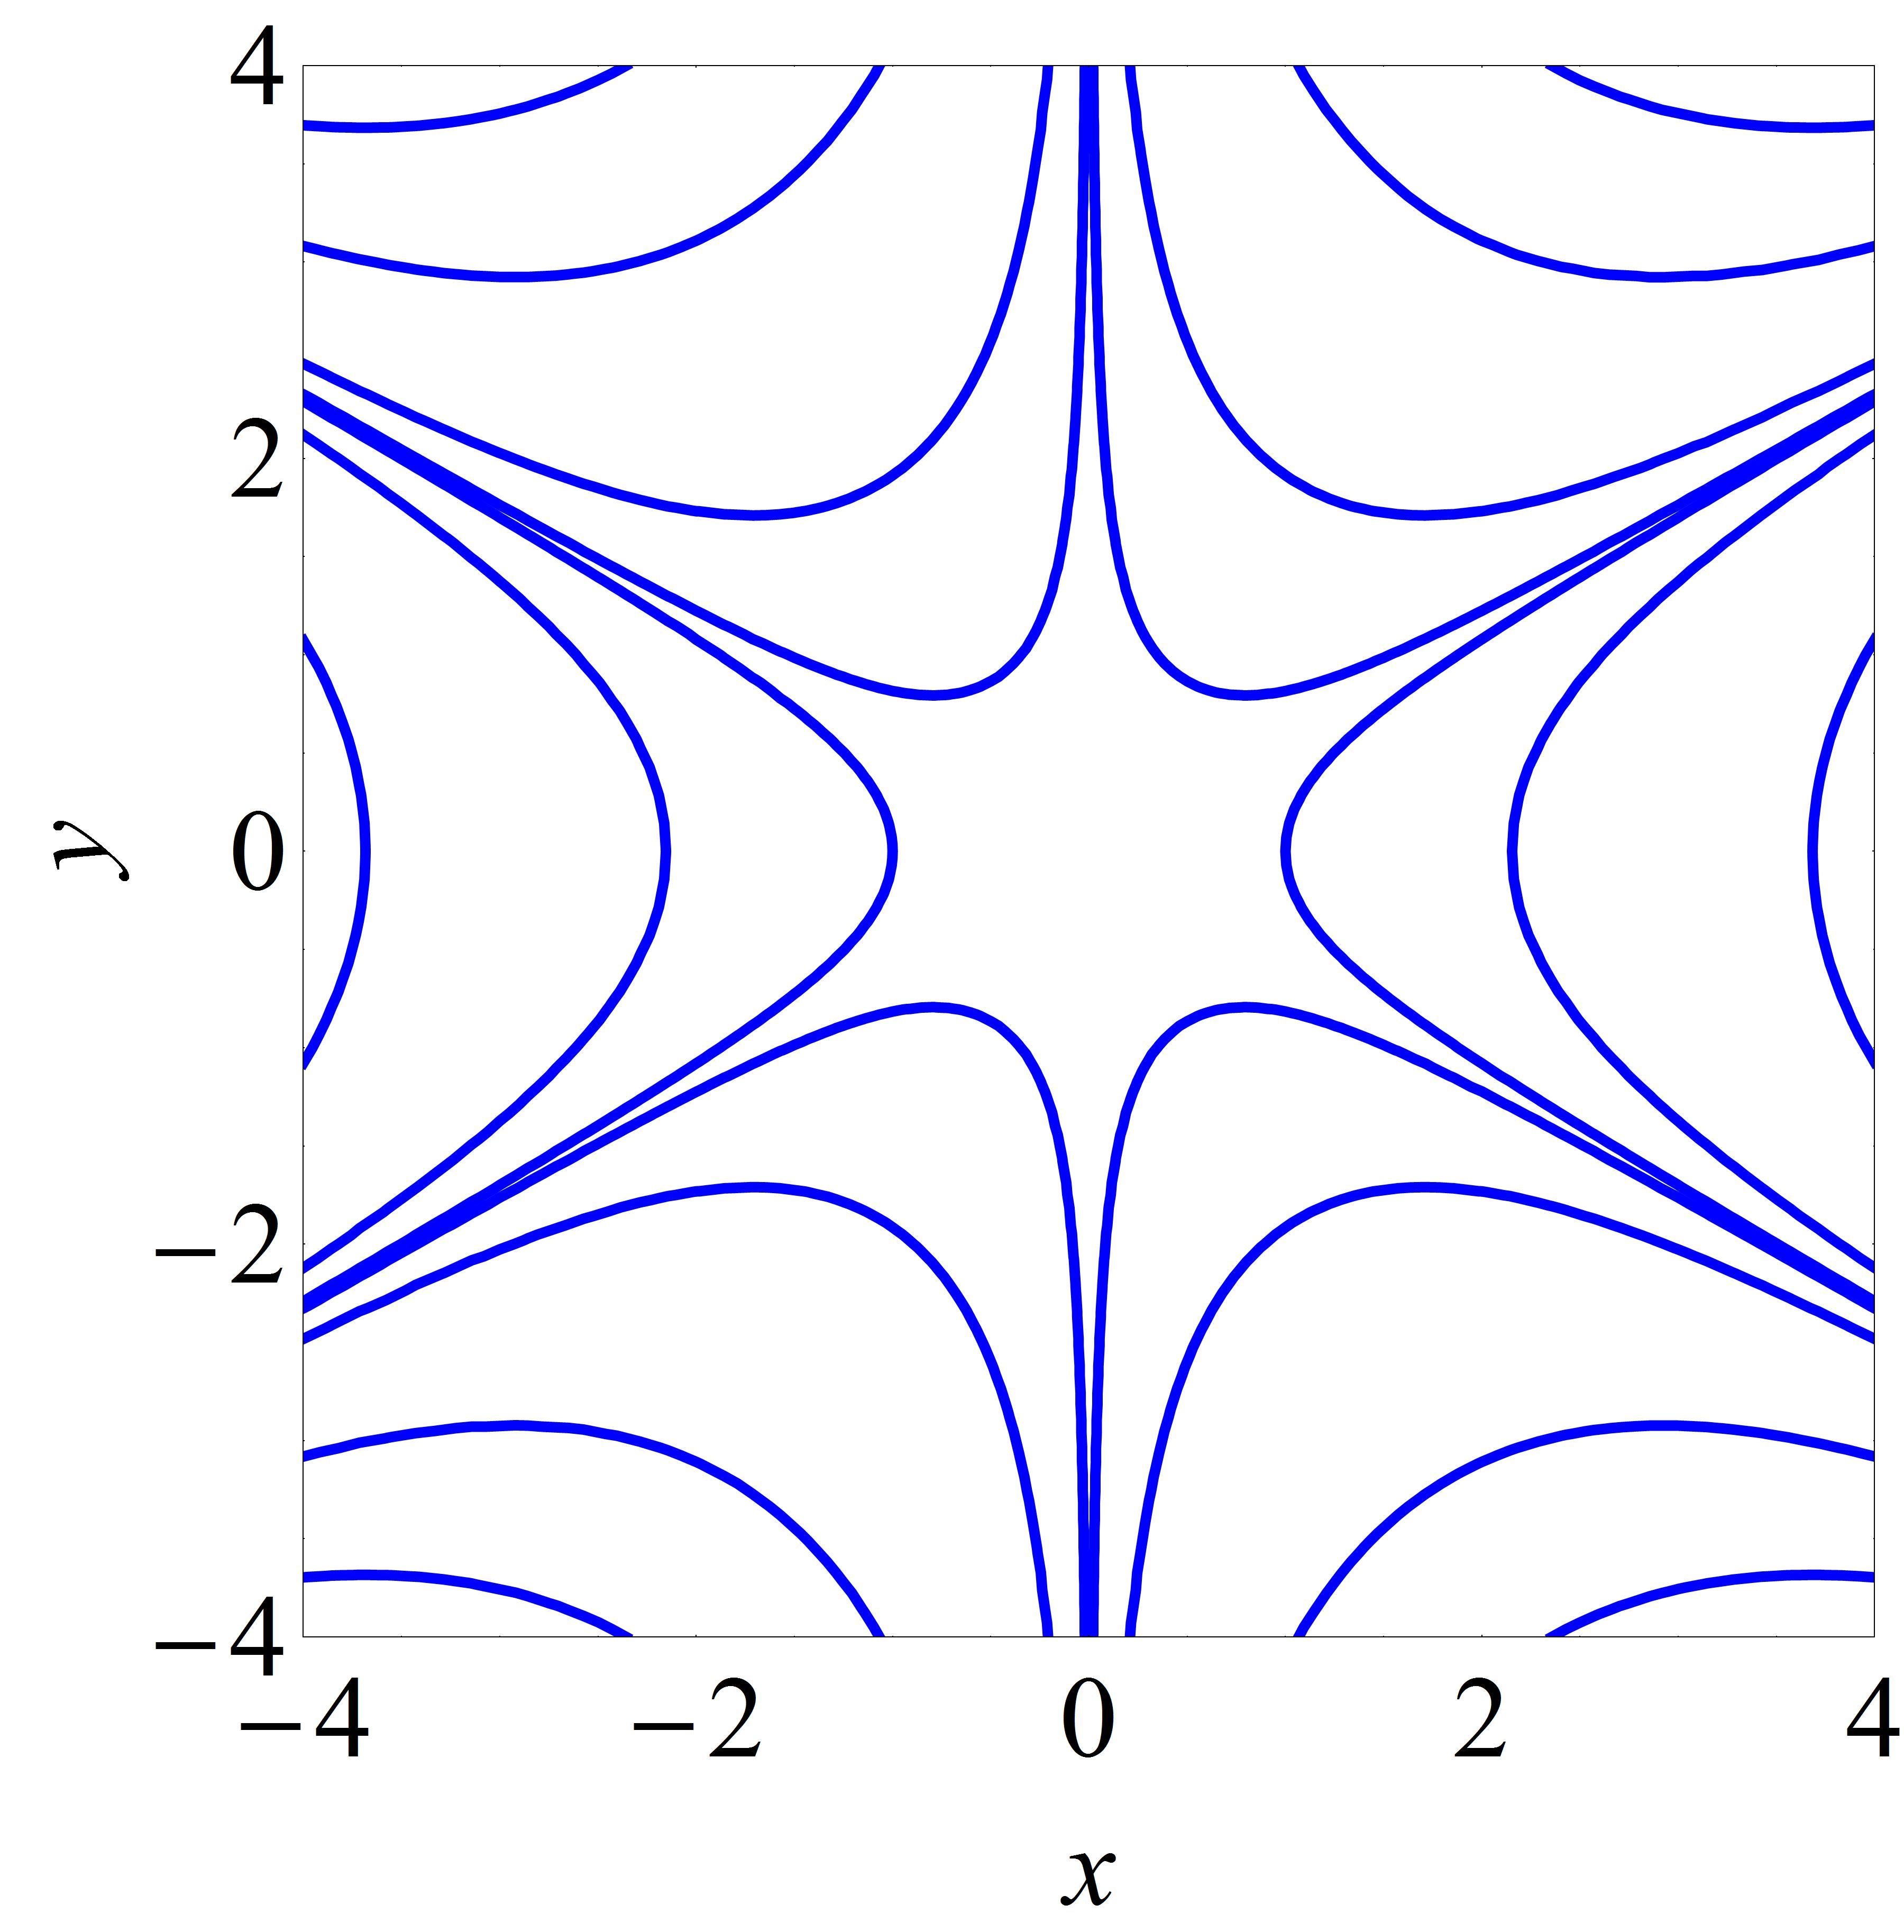
\includegraphics[height=4.5cm]{fig.jpg}\\
\caption{{\small Curvas de níveis da função $f(x,y)=x^3-3 x y^2$. }}
\label{niveis}
\end{figure}

{\bf IMPORTANTE:

O trabalho deve ser submetido via formulário que se encontra no site do evento.

Envie todos os arquivos necessários à produção do PDF em um único arquivo ZIP. Inclua o PDF compilado.
}


\section*{Seleção de trabalhos}

Os trabalhos submetidos, dentro do prazo estabelecido, serão enviados aos revisores do Comitê Científico. Com base nos pareceres do comitê, o trabalho poderá ser (1) aceito plenamente, (2) aceito sob a condição de que correções menores sejam feitas em curto prazo ou (3) rejeitado.


\section*{Citações}
Devem seguir as normas da ABNT NBR 10520. Nas citações, as chamadas pelo sobrenome do autor devem ser em letras maiúsculas e minúsculas e, quando estiverem entre parênteses, devem ser em letras maiúsculas.

Exemplos:

A ironia seria assim uma forma implícita de heterogeneidade mostrada, conforme a classificação proposta por Authier-Reiriz (1982).

\vskip 0.2cm
``Apesar das aparências, a desconstrução do logocentrismo não é uma psicanálise da filosofia [...]'' (DERRIDA, 1967, p. 293).

\vskip 0.2cm
a) As citações diretas, no texto, com mais de três linhas, devem ser destacadas com recuo de 4 cm da margem esquerda, espaço entre linhas simples e sem aspas, em fonte Times New Roman, tamanho 10.

\begin{quoting}
A teleconferência permite ao indivíduo participar de um encontro nacional ou regional sem a necessidade de deixar seu local de origem. Tipos comuns de teleconferência incluem o uso da televisão, telefone, e computador. Através de áudio-conferência, utilizando a companhia local de telefone, um sinal de áudio pode ser emitido em um salão de qualquer dimensão. (NICHOLS, 1993, p. 181).
\end{quoting}

\vskip 0.2cm
b) As citações diretas, no texto, de até três linhas, devem ser escritas entre ``aspas'' duplas e incorporadas ao texto.
Exemplos:
Barbour (1971, p. 35) descreve: ``O estudo da morfologia dos terrenos [...] ativos [...]''

\vskip 0.2cm
``Não se mova, faça de conta que está morta.'' (CLARAC; BONNIN, 1985, p. 72).

\vskip 0.2cm
Segundo Sá (1995, p. 27): ``[...] por meio da mesma `arte de conversação' que abrange tão extensa e significativa parte da nossa existência cotidiana [...]''

\vskip 0.2cm
c) Nas citações diretas, especificar no texto o ano de publicação e a(s) página(s) da fonte consultada. Estes dados devem ser colocados entre parênteses e separados por vírgula. Nas citações indiretas, a indicação da(s) página(s) consultada(s) é opcional, mas o ano de publicação da obra é obrigatório e deve estar entre parênteses.


\section*{Conclusões}

El crecimiento de un tumor puede ser visualizado en 3D utilizando la técnica de Marching Cubes. Se utiliza ampliamente para visualizaciones médicas, como imágenes de tomografía computarizada (TC) y resonancia magnética (RM). Además, el algoritmo de Marching Cubes puede reducir el tiempo de cálculo utilizado para el muestreo en la reconstrucción 3D. Sin embargo, uno de los problemas principales de Marching Cubes es la presencia de voxels no utilizados que pueden generarse durante el análisis de las coordenadas y los valores de intensidad de las imágenes 2D. Estos voxels no utilizados pueden afectar la suavidad de la superficie 3D ncbi.nlm.nih.gov.

\begin{figure}[h]
  \centering
  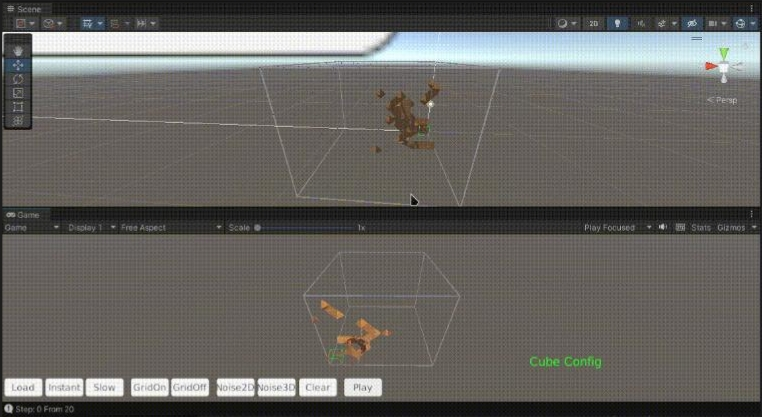
\includegraphics[width=0.9\textwidth]{tumor.jpg}
  \caption{Texto de la leyenda}
\end{figure}

La creación de una herramienta para simular el crecimiento de un tumor con un autómata celular en cualquier órgano del cuerpo humano es un avance significativo en el campo de la modelación y simulación de sistemas biológicos. Esta herramienta proporciona un enfoque innovador y flexible para estudiar el crecimiento de los tumores, lo cual tiene importantes implicaciones tanto en la investigación básica como en la clínica.

La capacidad de cargar configuraciones específicas y ajustar, agregar o eliminar parámetros que influyen en el realismo de la simulación permite adaptar el modelo a diferentes escenarios y condiciones. Esto hace que la herramienta sea altamente versátil y aplicable a una amplia gama de situaciones y tipos de tumores.

El uso de autómatas celulares para simular el crecimiento del tumor proporciona una representación detallada y dinámica del proceso. Los autómatas celulares son especialmente adecuados para este tipo de modelado, ya que permiten representar de forma precisa y realista la interacción entre las células y su entorno, así como los cambios que ocurren en el tiempo.

Finalmente, la visualización en 3D del crecimiento de un tumor utilizando la técnica de Marching Cubes puede proporcionar una herramienta valiosa para los profesionales de la salud para entender mejor la dinámica del crecimiento del tumor y desarrollar estrategias de tratamiento más efectivas.

\section*{Agradecimentos}

Os autores podem apresentar os agradecimentos a pessoas e instituições. Esta seção é OPCIONAL.



%%%%%%%%%%%%%%%%%%%%%%%%%%%%%
%%%%%%%%%%%%%%%%%%%%%%%%%%%%%

\section*{Referências}
{\color{red} A bibliografia deverá seguir o padrão da ABNT NBR 6023, separadas entre si por uma linha em branco, estar em \textbf{ordem alfabética pelo sobrenome do primeiro autor}, se necessário, usando-se, ainda, ordem cronológica, para trabalhos de um mesmo autor. Trabalhos dos mesmos autores, publicados no mesmo ano, devem ser listados utilizando-se a ordem alfabética do título do trabalho. Basicamente, as referências devem conter as iniciais dos nomes dos autores, sendo escrito, por extenso, apenas o último sobrenome. Seguem alguns exemplos:}


\begin{flushleft}

\begin{thebibliography}{99}
\bibitem{1} V Guinot. Modelling using stochastic, finite state cellular automata: rule inference from continuum models. Applied Mathematical Modelling, 26(6)\\
\bibitem{2} H. Ruanxiaogang. A simple cellular automaton model for tumor-immunity system. Robotics, Intelligent Systems and Signal Processing, 2003. Proceedings. 2003 IEEE International Conference on, 2\\
\bibitem{3} A. Deutsch, P. Maini, and S. Dormann. Cellular Automaton Modeling of Biological Pattern Formation: Characterization, Applications, and Analysis. Modeling and Simulation in Science, Engineering and Technology. Birkhauser Boston, 2007.\\
\bibitem{4} A. Kansal and S. Torquato. Simulated brain tumor growth dynamics using a three-dimentional cellular automaton. Journal of Theoretical Biology
\bibitem{5} Autor: Darien Viera Barredo. Instituci\'on: Universidad de La Habana, Facultad de Matem\'atica y Computaci\'on. Departamento de Matem\'atica. Asesores: Reinaldo Rodr\'iguez Ramos, Rub\'en Interi\'an, Ariel Ram\'irez Torres, Roc\'io Rodr\'iguez S\'anchez. A\~no: June, 2019.
\bibitem{6} https://journal-bcs.springeropen.com/articles/10.1007/s13173-012-0097-z

\bibitem{7} https://en.wikipedia.org/wiki/Marching_cubes

\bibitem{8} https://ncbi.nlm.nih.gov/pmc/articles/PMC8321043

\end{thebibliography}

%Livro com até 3 autores:

GAUTSCHI, W. A survey of gauss-christoffel quadrature formulae. In: BUTZER, P.L.; FEHER, F. (Edit.). {\bf E. B. Christoffel: the influence of his work on mathematics and the physical sciences}. Basel; Boston: Birkhauser Verlag, 1981. p. 72-147.

\vskip 0.2cm
BRUNETTI, F. \textbf{Mecânica dos fluidos}. 2.ed. São Paulo:Pearson, 2005.

\vskip 0.2cm
JAIN, A.; ROSS, A.; NANDAKUMAR, K. \textbf{Introduction to Biometrics}. 1. ed. New York: Springer, 2001.

\vskip 0.2cm

%Livro com 4 autores ou mais:

ARENALES, M. et al. \textbf{Pesquisa Operacional}. Rio de Janeiro: Elsevier, 2006.

\vskip 0.2cm

%Artigo em periódico:

AVILA, A. Density of positive Lyapunov Exponents for $SL(2,\mathbb{R})$ cocycles. \textbf{Journal of the America Mathematical Society}, v. 24, n.4, p. 999-1014, 2011.

\vskip 0.2cm

KURODA, L. K. B. et al. Método da transformada diferencial generalizada no modelo fracionário de Malthus. \textbf{C.Q.D. - Revista Eletrônica Paulista de Matemática}, Bauru, v. 10, p. 68-78, dez. 2017. Edição Ermac. 

\vskip 0.2cm

%Trabalho em evento:

BRAYNER, A. R. A.; MEDEIROS, C. B. Incorporação do tempo em SGBD orientado a objetos. In: SIMPÓSIO BRASILEIRO DE BANCO DE DADOS, 9., 1994, São Paulo. \textbf{Anais...} São Paulo: USP, 1994. p. 16-29.

\vskip 0.2cm

%Dissertações e teses:

CHERRI, A.C. \textbf{Reaprendendo tópicos de cálculo diferencial com o auxilio de softwares matemáticos}. 2001. 154 f. Trabalho de Conclusão de Curso (Especialização) \textendash\ Faculdade de Ciências, UNESP, Bauru, 2001.

\vskip 0.2cm
DINIZ,G. L. \textbf{A mudança no habitat de populações de peixes: de rio a represa -- o modelo
matemático}. 1994. 90 f. Dissertação (Mestrado em Matemática Aplicada) \textendash\ Unicamp, Campinas, 1994.

\vskip 0.2cm
OLIVEIRA, E.L. \textbf{Torres de Extensões Abelianas
de grau primo ímpar não ramificado}.2015. 63f. Tese (Doutorado em Matemática) \textendash\ IBILCE/UNESP, São José do Rio Preto, 2015.

\vskip 0.2cm

%Homepages:

INTERNATIONAL GEOGEBRA INSTITUTE. Matemática dinâmica para se aprender e se ensinar. 2014. Disponível em: http://www.geogebra.org/cms. Acesso em: 17 dez. 2014.
\end{flushleft}

\end{document}
